\section{Architektur und Komponenten}\label{sec:architektur-und-komponenten}

Das Evaluationsframework ist modular aufgebaut und nutzt eine Pipeline-Architektur, um eine flexible und skalierbare Evaluierung zu ermöglichen. Die Architektur ist in Abbildung~\ref{fig:evaluation-framework-architecture} dargestellt. Sie besteht aus mehreren Hauptkomponenten, die jeweils eine klar definierte Aufgabe erfüllen und über wohldefinierte Schnittstellen miteinander kommunizieren. Im Folgenden werden die Komponenten und ihr Zusammenspiel beschrieben.

\subsection*{Einstiegspunkte}

Das Framework bietet zwei Einstiegspunkte zur Ausführung einer Evaluierung:

\begin{itemize}
    \item \textbf{EvaluationController}: Dieser HTTP-Controller stellt REST-Endpunkte bereit, über die Evaluierungen gestartet werden können. Er akzeptiert eine \texttt{MultiEvaluationRequest}-Konfiguration und gibt die Ergebnisse entweder als Markdown-Bericht oder als JSON-Stream zurück. Der Controller ist in das Spring-Boot-Backend integriert und ermöglicht die Nutzung des Frameworks über die Weboberfläche sowie über HTTP-APIs.
    \item \textbf{EvaluationCommand}: Dieser CLI-Befehl erlaubt die Ausführung von Evaluierungen über die Kommandozeile. Er liest eine YAML-Konfigurationsdatei ein, führt die Evaluierung aus und schreibt die Ergebnisse in eine Markdown-Datei. Dies eignet sich besonders für automatisierte Ausführungen, Continuous Integration oder die lokale Entwicklung.
\end{itemize}

Beide Einstiegspunkte nehmen dieselbe \texttt{MultiEvaluationRequest}-Konfiguration entgegen und delegieren die Ausführung an die Kernkomponente \texttt{MultiEvaluationRunner}.

\subsection*{Orchestrierung mit MultiEvaluationRunner}

Der \texttt{MultiEvaluationRunner} ist für die Orchestrierung der gesamten Evaluierung verantwortlich. Er verarbeitet eine \texttt{MultiEvaluationRequest}, die mehrere Modelle und Datensätze beschreibt, und koordiniert die sequenzielle Evaluierung aller konfigurierten Modelle. Für jedes Modell erzeugt der \texttt{MultiEvaluationRunner} eine separate \texttt{EvaluationRequest} und übergibt diese an den \texttt{EvaluationRunner}.

Der \texttt{MultiEvaluationRunner} stellt zudem sicher, dass alle Modelle denselben Seed verwenden, um reproduzierbare Ergebnisse zu gewährleisten. Er sammelt die Metadaten über die verwendeten Datensätze, Modelle und Endpunkte und gibt diese als Teil des Evaluationsberichts zurück. Die Ergebnisse werden als \texttt{Flow} von \texttt{ModelReportEnvelope}-Objekten zurückgegeben, wodurch eine streambasierte Verarbeitung ermöglicht wird.

\subsection*{Ausführung mit EvaluationRunner}

Der \texttt{EvaluationRunner} führt die Evaluierung für ein einzelnes Modell durch. Er lädt die Testdatensätze aus der Datenbank, führt die Klassifizierung für jeden Testfall aus und sammelt die Ergebnisse. Die Testfälle werden parallel verarbeitet, wobei die Anzahl der gleichzeitigen Ausführungen durch den Parameter \texttt{maxConcurrent} in der Konfiguration gesteuert wird. Dies ermöglicht es, Rate-Limits von \acp{LLM}-Diensten einzuhalten und die Auslastung der Ressourcen zu kontrollieren.

Für jeden Testfall delegiert der \texttt{EvaluationRunner} die eigentliche Klassifizierung an den \texttt{HttpEvaluator}. Anschließend vergleicht er die erwarteten mit den tatsächlichen Ergebnissen und berechnet die Klassifikationsmetriken (True Positives, False Positives, False Negatives, True Negatives). Die Ergebnisse werden in \texttt{TestCaseReport}-Objekten zusammengefasst und an den \texttt{MetricsAccumulator} weitergeleitet.

Der \texttt{EvaluationRunner} gibt die Ergebnisse als \texttt{Flow} zurück, wodurch eine frühzeitige Rückgabe ermöglicht wird. Dies ist besonders vorteilhaft für die Live-Ansicht in der Weboberfläche, da Testfallergebnisse sofort nach ihrer Fertigstellung angezeigt werden können.

\subsection*{Klassifizierung mit HttpEvaluator}

Der \texttt{HttpEvaluator} ist für die Kommunikation mit dem Klassifizierungsendpunkt verantwortlich. Er nimmt ein \ac{BPMN}-Modell entgegen, baut einen HTTP-Request auf und sendet diesen an den konfigurierten Endpunkt. Der Endpunkt kann entweder lokal (z.B. ein anderer Controller im selben Backend) oder extern (z.B. ein separater Dienst) sein.

Der \texttt{HttpEvaluator} fügt die \texttt{llmProps} aus der Konfiguration als Teil des Requests hinzu, wodurch Modell-spezifische Parameter wie \texttt{modelName}, \texttt{apiKey} und \texttt{seed} übermittelt werden. Nach erfolgreicher Klassifizierung extrahiert er die Liste der als kritisch identifizierten Aktivitäten aus der Antwort und gibt diese als \texttt{List<ExpectedValue>} zurück.

\subsection*{Akkumulierung mit MetricsAccumulator}

Der \texttt{MetricsAccumulator} sammelt die Metriken aller Testfälle eines Modells und berechnet daraus aggregierte Werte. Er ist thread-sicher implementiert und kann gleichzeitig von mehreren parallelen Evaluierungen genutzt werden.

Nach Abschluss aller Testfälle erzeugt der \texttt{MetricsAccumulator} ein \texttt{EvaluationReportSummary}-Objekt, das die folgenden Metriken enthält:

\begin{itemize}
    \item \textbf{Anzahl Testfälle}: Gesamtzahl, erfolgreich, fehlgeschlagen und mit Fehlern
    \item \textbf{Precision}: Anteil der korrekt als kritisch klassifizierten Aktivitäten an allen als kritisch klassifizierten Aktivitäten
    \item \textbf{Recall}: Anteil der korrekt als kritisch klassifizierten Aktivitäten an allen tatsächlich kritischen Aktivitäten
    \item \textbf{F1-Score}: Harmonisches Mittel aus Precision und Recall
    \item \textbf{Accuracy}: Anteil der korrekt klassifizierten Aktivitäten an allen Aktivitäten
    \item \textbf{Konfusionsmatrix}: True Positives, False Positives, False Negatives, True Negatives
\end{itemize}

\subsection*{Datenfluss}

Der Datenfluss durch das Framework verläuft wie folgt:

\begin{enumerate}
    \item Ein Nutzer startet eine Evaluierung über den \texttt{EvaluationController} (HTTP) oder \texttt{EvaluationCommand} (CLI) und übergibt eine \texttt{MultiEvaluationRequest}-Konfiguration.
    \item Der \texttt{MultiEvaluationRunner} liest die Konfiguration ein, lädt Metadaten über die Datensätze und iteriert über alle konfigurierten Modelle.
    \item Für jedes Modell übergibt der \texttt{MultiEvaluationRunner} eine \texttt{EvaluationRequest} an den \texttt{EvaluationRunner}.
    \item Der \texttt{EvaluationRunner} lädt die Testdaten aus der Datenbank und verarbeitet jeden Testfall parallel. Dabei wird die Nebenläufigkeit durch \texttt{maxConcurrent} gesteuert.
    \item Für jeden Testfall ruft der \texttt{EvaluationRunner} den \texttt{HttpEvaluator} auf, der die Klassifizierung über einen HTTP-Endpunkt durchführt.
    \item Die Ergebnisse der Klassifizierung werden mit den erwarteten Werten verglichen, und die Metriken werden berechnet.
    \item Die Testfallergebnisse werden an den \texttt{MetricsAccumulator} weitergeleitet und als \texttt{TestCaseReport} zurückgegeben.
    \item Nach Abschluss aller Testfälle eines Modells erstellt der \texttt{MetricsAccumulator} ein \texttt{EvaluationReportSummary} mit den aggregierten Metriken.
    \item Der \texttt{MultiEvaluationRunner} verpackt alle Ergebnisse in \texttt{ModelReportEnvelope}-Objekte und gibt diese als Stream zurück.
    \item Die Ergebnisse werden vom Einstiegspunkt (Controller oder CLI) weiterverarbeitet und ausgegeben.
\end{enumerate}

Diese Pipeline-Architektur ermöglicht eine flexible Erweiterung des Frameworks, beispielsweise durch Austausch des \texttt{HttpEvaluator} gegen andere Evaluatoren oder durch Hinzufügen zusätzlicher Metriken im \texttt{MetricsAccumulator}.

\begin{figure}
    \centering
    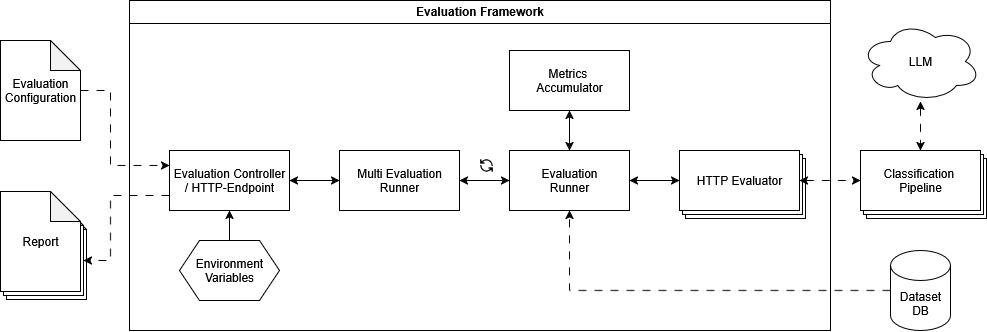
\includegraphics[width=.9\linewidth]{images/evaluation/evaluation-framework-architecture}
    \caption{Architektur des Evaluationsframeworks}
    \label{fig:evaluation-framework-architecture}
\end{figure}